\begin{titlepage}
  \begin{center}

  {\Huge BUS SPI MASTER}

  \vspace{25mm}

  
\includegraphics[width=0.90\textwidth,height=\textheight,keepaspectratio]{img/AFRL.png}

  \vspace{25mm}

  \today

  \vspace{15mm}

  {\Large Jay Convertino}

  \end{center}
\end{titlepage}

\tableofcontents

\newpage

\section{Usage}

\subsection{Introduction}

\par
BUS SPI Master core emulates and extends the Altera SPI IP core. This is a SPI master device only. It is
currently available as a AXI Lite, Wishbone Standard, and uP bus IP core. The Altera core this is based on has Linux
and uboot drivers, by mimicking it this core has instant access to its support software. There is a extension register for control
that allows for changes to the SPI Master the Altera IP does not have. The CPOL/CPOH can be changed. A new speed registers
controls the speed of the device outside of the initial setting. The following is information on how to use the
device in an FPGA, software, and in simulation.

\subsection{Dependencies}

\par
The following are the dependencies of the cores.

\begin{itemize}
  \item fusesoc 2.X
  \item iverilog (simulation)
  \item cocotb (simulation)
\end{itemize}

\subsubsection{axi\_lite\_spi\_master Depenecies}
\begin{itemize}
\item dep
	\begin{itemize}
	\item AFRL:utility:helper:1.0.0
	\item AFRL:device:up\_spi\_master:1.0.0
	\item AD:common:up\_axi:1.0.0
	\end{itemize}
\item dep\_tb
	\begin{itemize}
	\item AFRL:simulation:axis\_stimulator
	\item AFRL:utility:sim\_helper
	\end{itemize}
\end{itemize}


\subsubsection{wishbone\_standard\_spi\_master Depenecies}
\begin{itemize}
\item dep
	\begin{itemize}
	\item AFRL:utility:helper:1.0.0
	\item AFRL:device:up\_spi\_master:1.0.0
	\item AFRL:bus:up\_wishbone\_standard:1.0.0
	\end{itemize}
\end{itemize}


\subsubsection{up\_spi\_master Depenecies}
\begin{itemize}
\item dep
	\begin{itemize}
	\item AFRL:utility:helper:1.0.0
	\item AFRL:device\_converter:axis\_spi\_master:1.0.0
	\item AFRL:buffer:axis\_fifo:1.0.0
	\end{itemize}
\end{itemize}


\subsection{In a Project}
\par
First, pick a core that matches the target bus in question. Then connect the BUS SPI MASTER core to that bus. Once this is complete the SPI pins will need to be routed to the slave SPI devices. The core can be used with a 32 bit or 16 bit databus (4 or 2 bytes). Any other size is not supported and will result in a core that acts strange or don't build at all.

\section{Architecture}
\par
This core is made up of other cores that are documented in detail in their source. The cores this is made up of are:
\begin{itemize}
  \item \textbf{axis\_spi\_master} Interface with SPI master and present the data over AXIS interface (see core for documentation).
  \item \textbf{up\_axi} An AXI Lite to uP converter core (see core for documentation).
  \item \textbf{up\_wishbone\_standard} A wishbone standard to uP converter core (see core for documentation).
  \item \textbf{up\_spi\_master} Takes uP bus and coverts it for interfacing with the AXIS SPI core (see module documentation for information \ref{Module Documentation}).
\end{itemize}

\subsection{Registers}
For register bit documentation please see up\_spi\_master subsetion registers in \ref{Module Documentation}

\par
Interrupts for this core are enabled in the control register. First the general error IE bit, interrupt enable for all errors, is set to 1.
All errors will now generate a interrupt. IOE, IROE, etc will not need to be activated. This interrupt goes active high (1) when a condition becomes
true. Starting with the interrupt end of packet bit (IEOP), setting this active will enable the interrupt to go off when the status EOP bit
is true. This will stay that way till the tx or rx register is cleared of the EOP word. Interrupt read ready (IRRDY) when set active will trigger
an interrupt when the status bit RRDY is active. This will stay tripped till a word is read. Interrupt transmit ready (ITRDY) when set active will
trigger an interrupt when the status bit TRDY is active. This will stay tripped till a word is written. Interrupt transmit overrun (ITOE) when set
active will trigger an interrupt when the status bit TOE is active. This will stay tripped till the status register is written. Interrupt receive
underrun (IROE) when set active will trigger an interrupt when the status bit ROE is active. ITOE, TOE, IROE, ROE, and E are only cleared by writing to the
status register. The status register does NOT write any actual data to the register, status bits are not directly affected. It simply
resets ROE/TOE to 0. See \ref{Module Documentation} up\_spi\_master for more detail on the location and function of register bits.

\subsection{Waveforms}
The idealized simulation waveforms are shown below. The values reflect the results of using the icarus backend with surfer view tools.

\par
Write slave is the first uP test that looks at writing to a slave device using the SPI master without reading the received data.
\begin{figure}[H]
\caption{write slave uP}
\centering
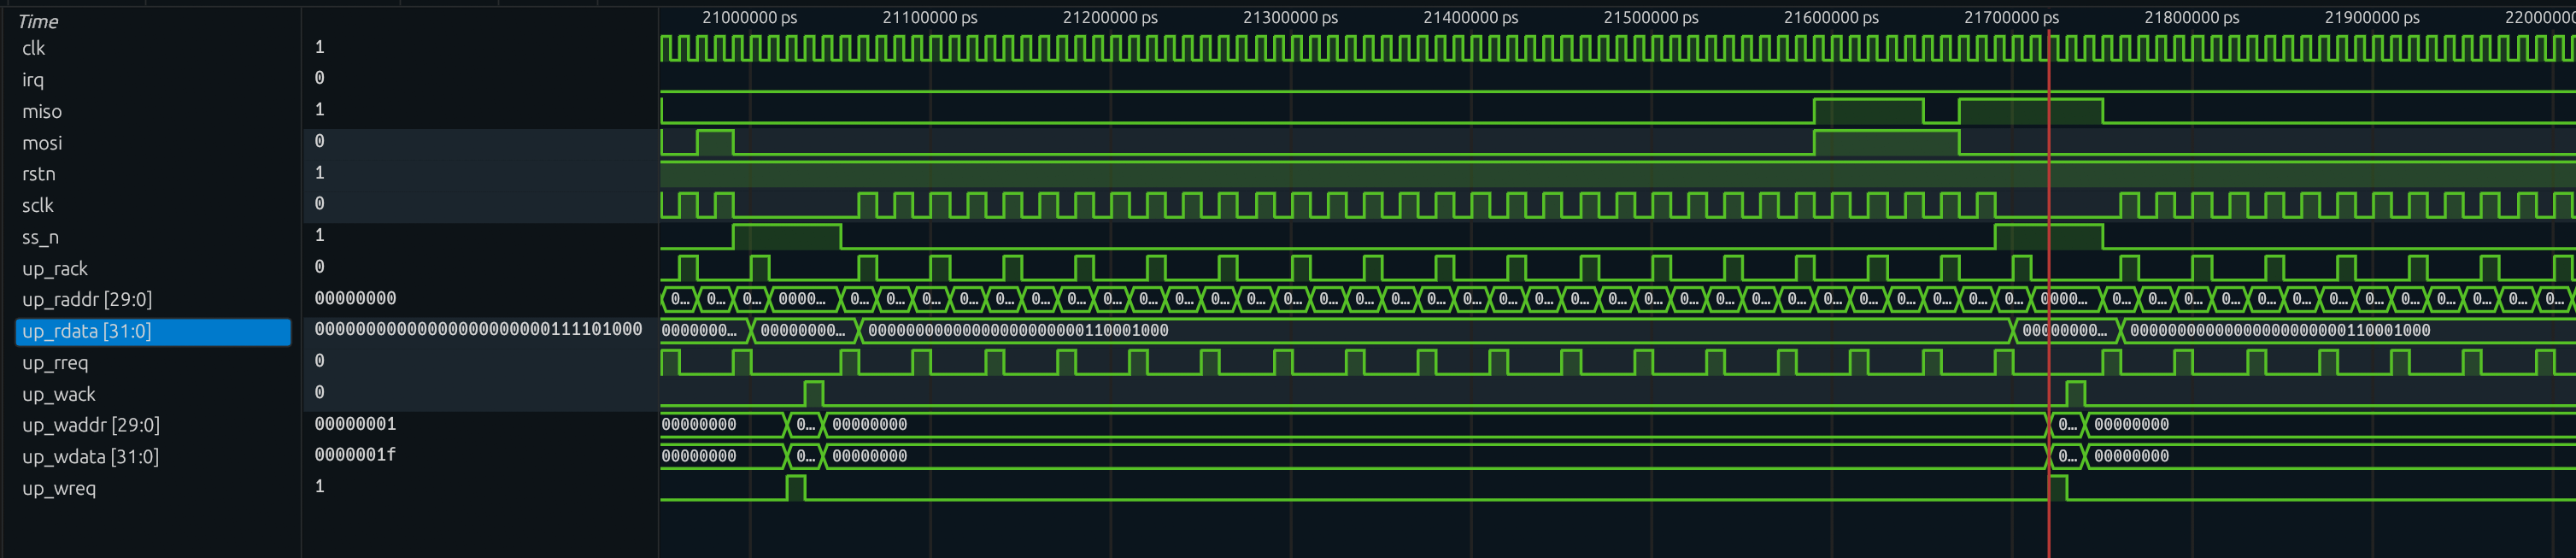
\includegraphics[width=\textwidth]{img/diagrams/waveform_write_slave_up.png}
\end{figure}

\par
Loop test checks for reads and writes on the uP bus.
\begin{figure}[H]
\caption{loop test uP}
\centering
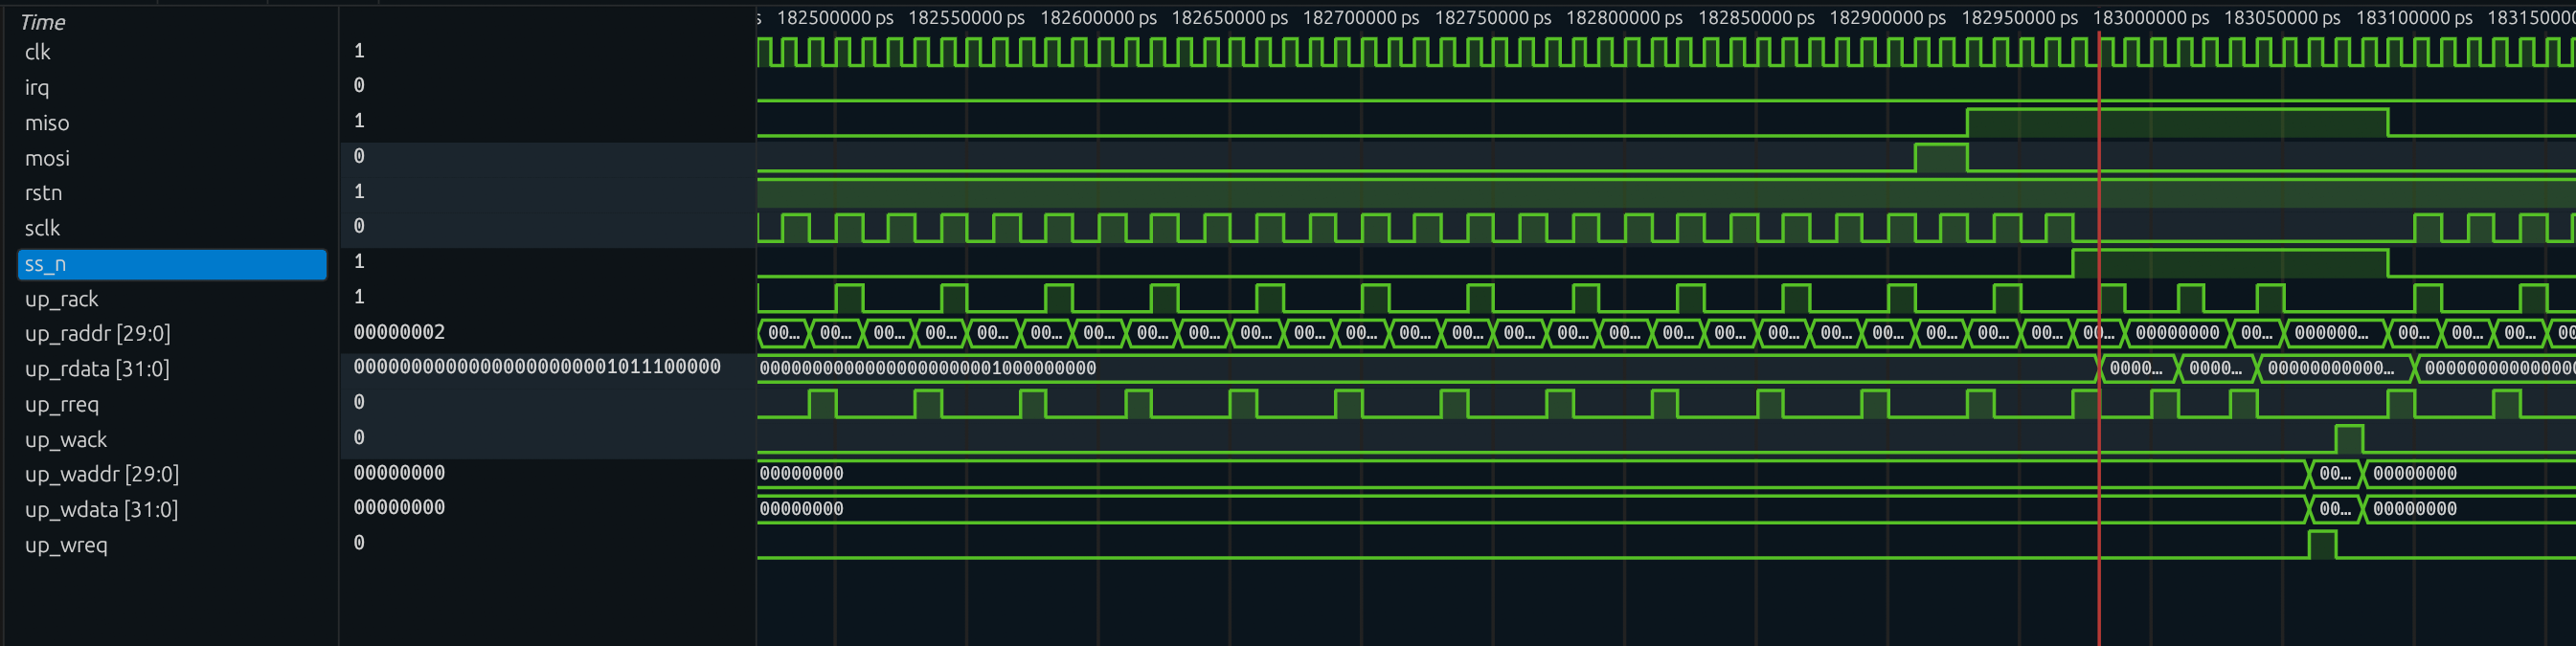
\includegraphics[width=\textwidth]{img/diagrams/waveform_loop_test_up.png}
\end{figure}

\par
Next are various interrupt enable tests to see if they respond as they should.
\begin{figure}[H]
\caption{read ready interrupt enabled}
\centering
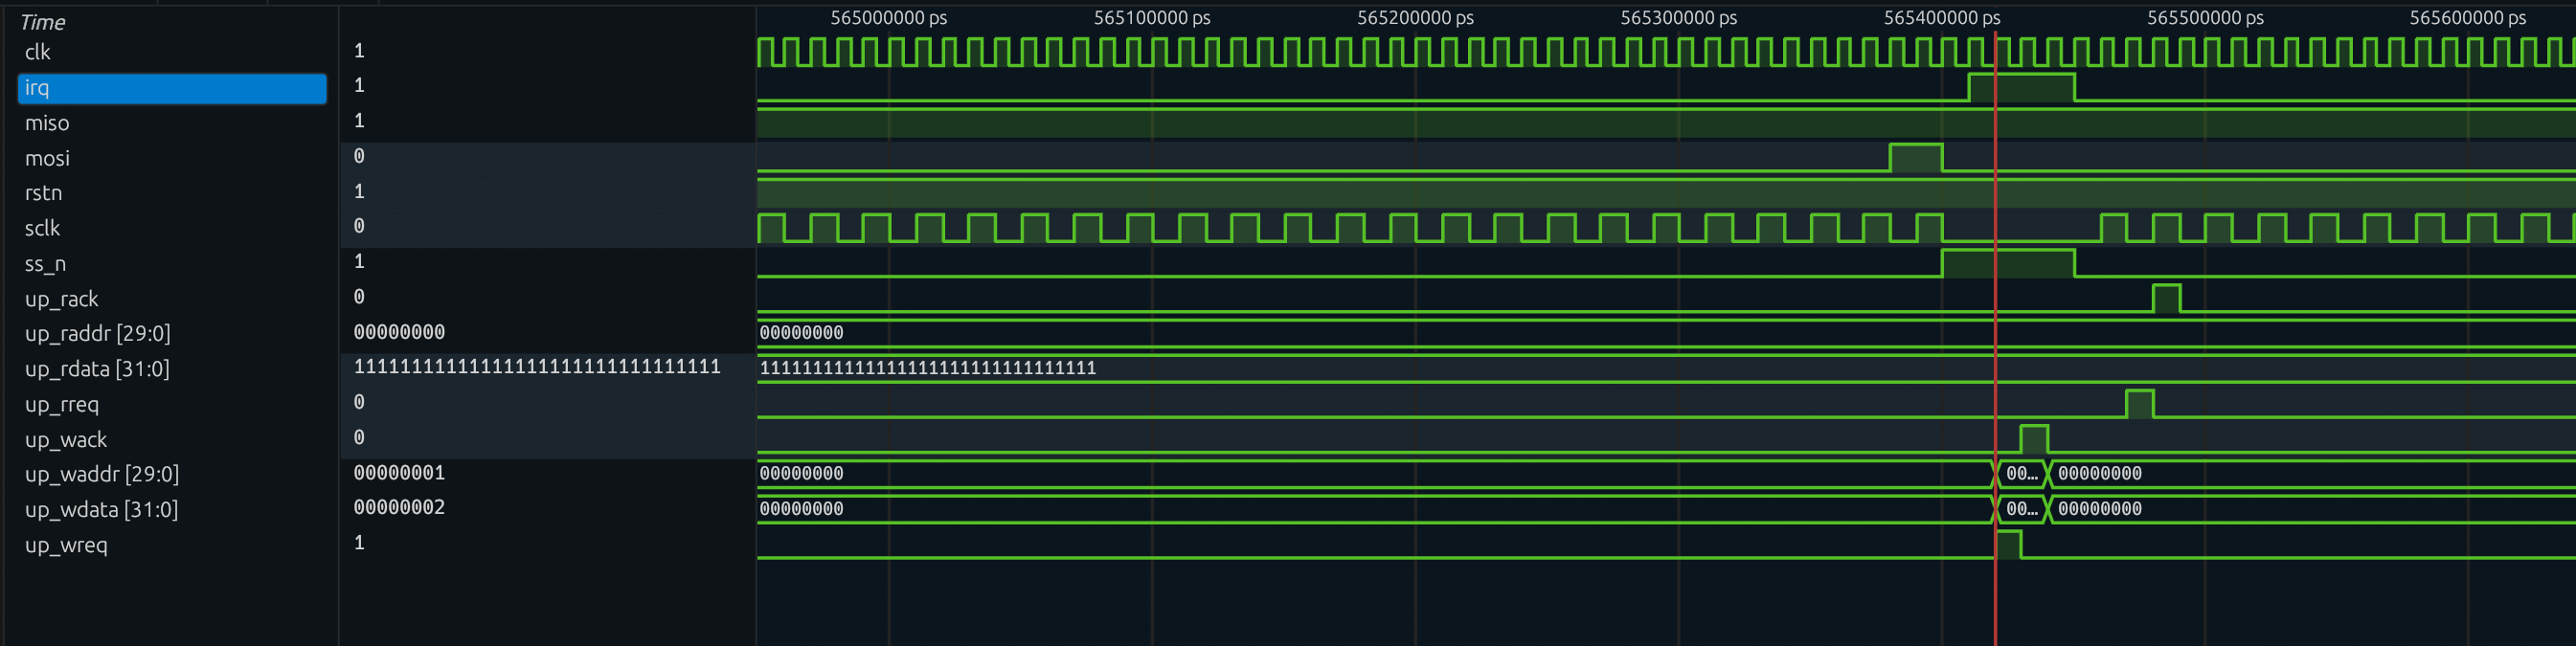
\includegraphics[width=\textwidth]{img/diagrams/waveform_irrdy_up.png}
\end{figure}

\begin{figure}[H]
\caption{transmit error interrupt enabled}
\centering
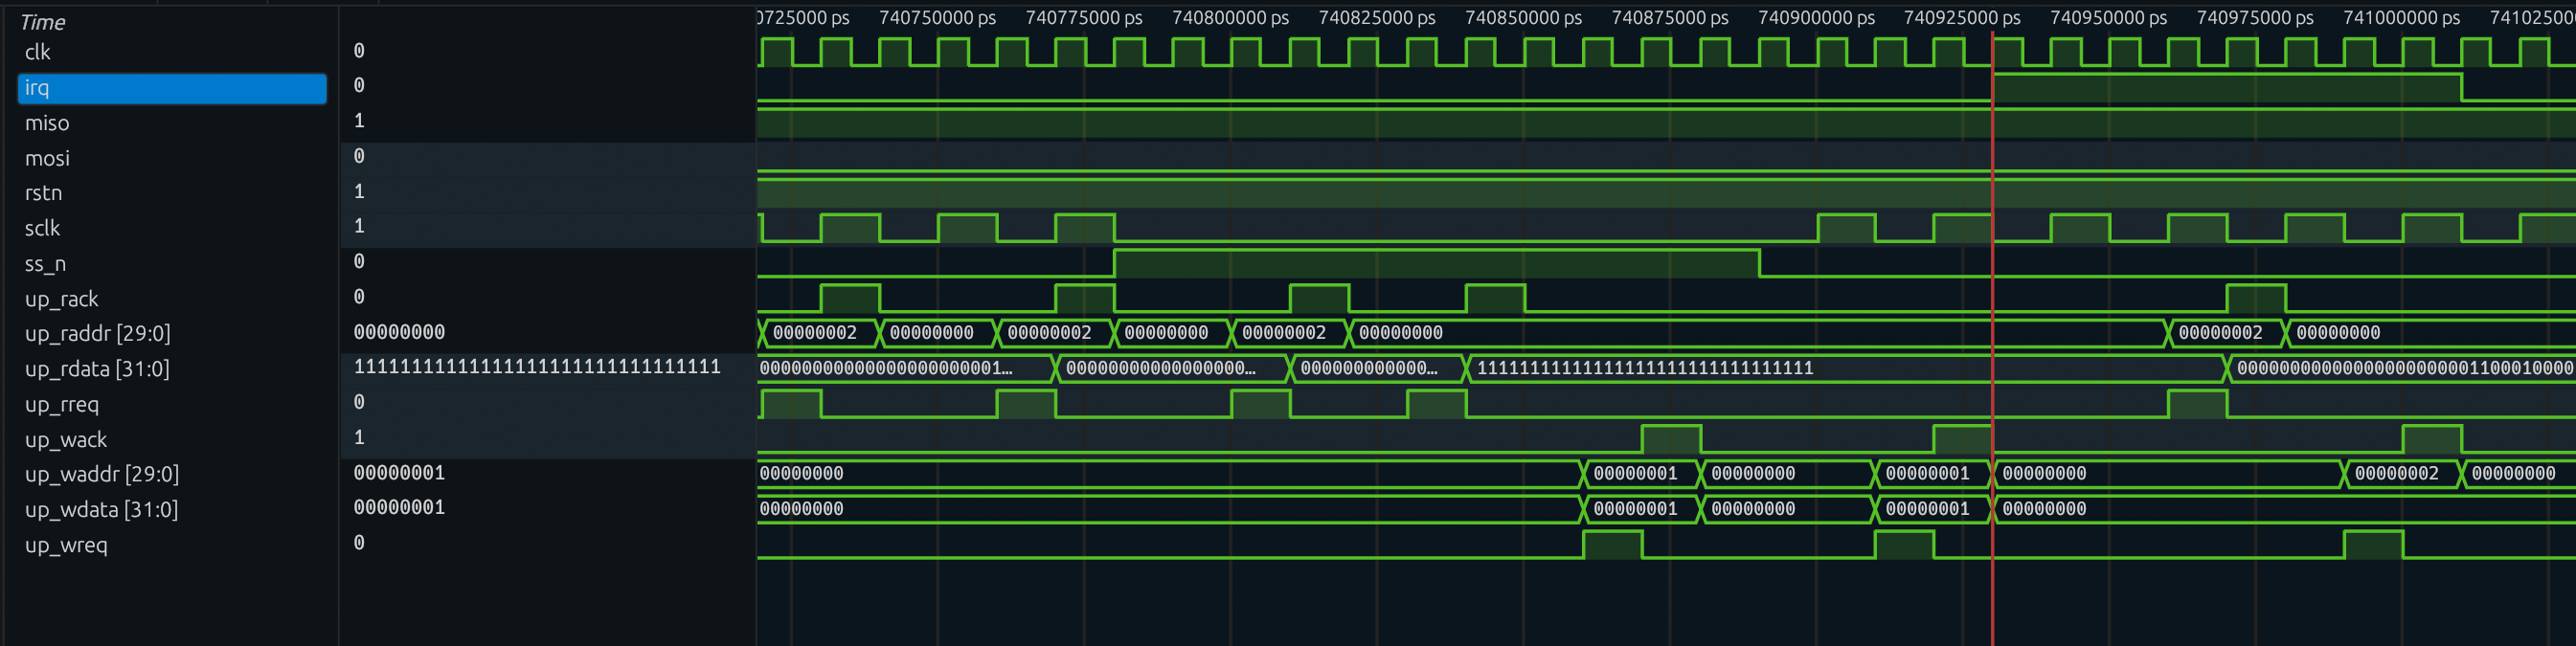
\includegraphics[width=\textwidth]{img/diagrams/waveform_itoe_up.png}
\end{figure}

\par
End of packet is a feature added to the Altera IP core in 2019. It is not present in the linux drivers.
Its functionality is questionable when it comes to being useful. Essentially it allows the device to signal
bits or a irq if a EOP word matches the transmit or receive register contents. It is cleared when those
contents change and are not the EOP.
\begin{figure}[H]
\caption{EOP}
\centering
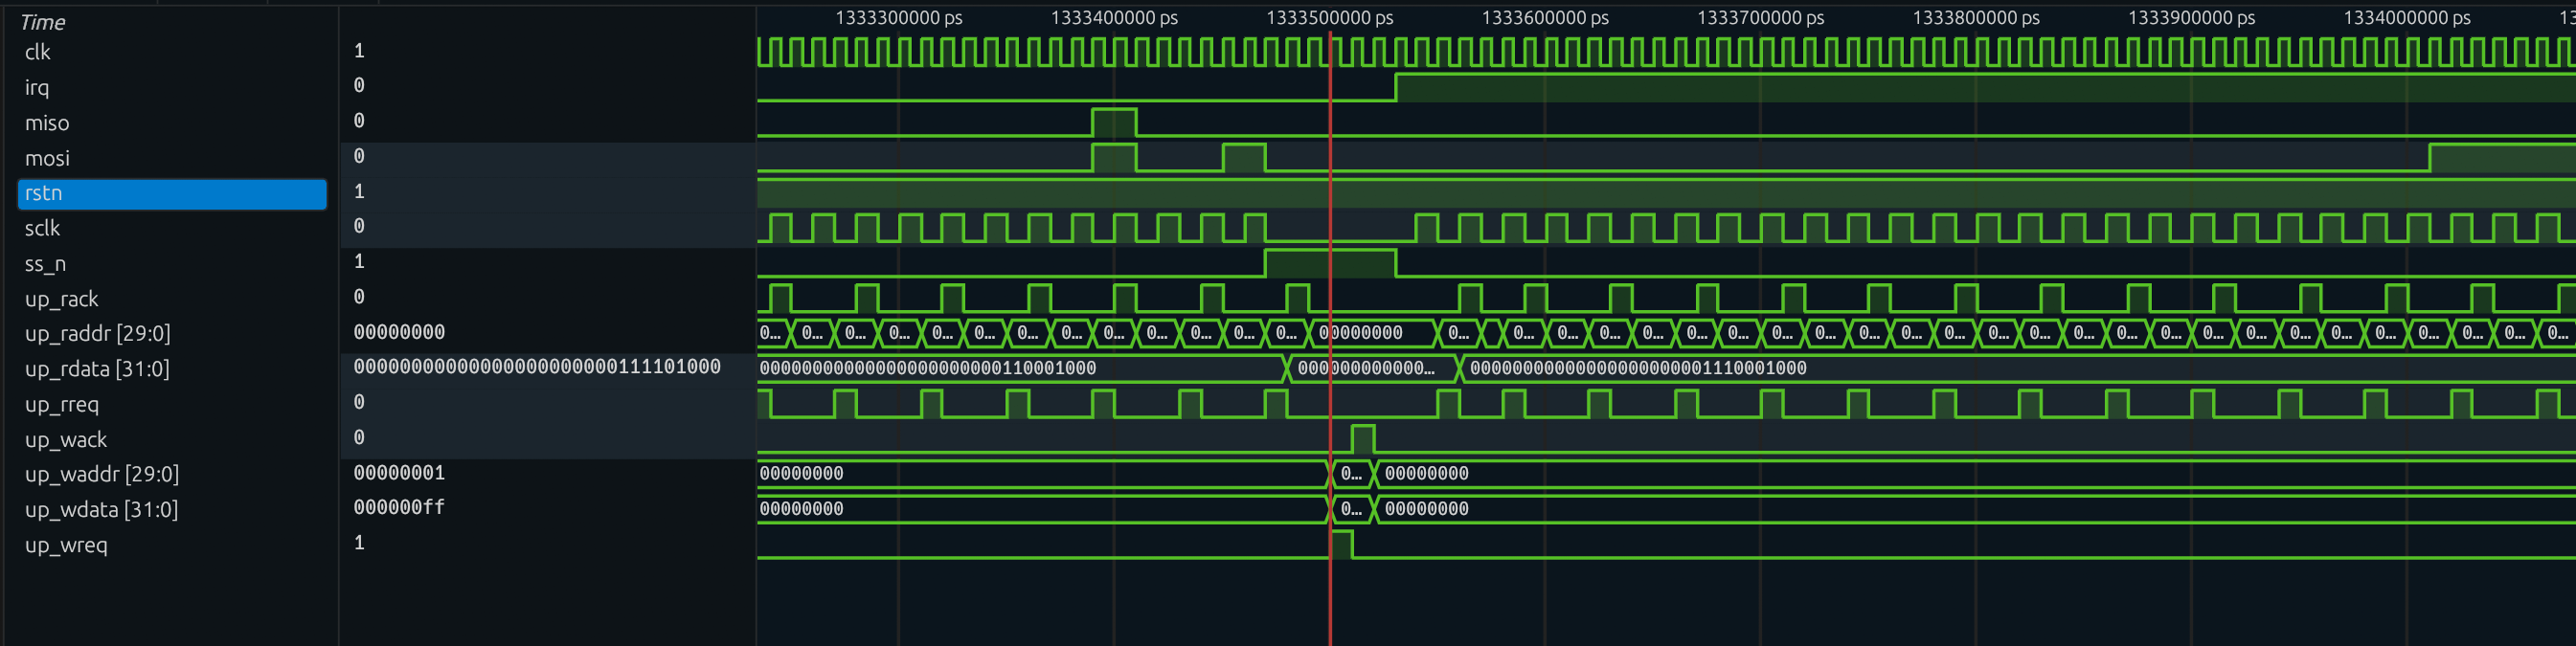
\includegraphics[width=\textwidth]{img/diagrams/waveform_eop_up.png}
\end{figure}

\par
The last two waveforms show the uP to bus adapters in a loopback test. Since it takes two writes to get the SPI slave to
echo a value written in two previous writes, the read value will be two writes behind.
\begin{figure}[H]
\caption{loop test AXI Lite}
\centering
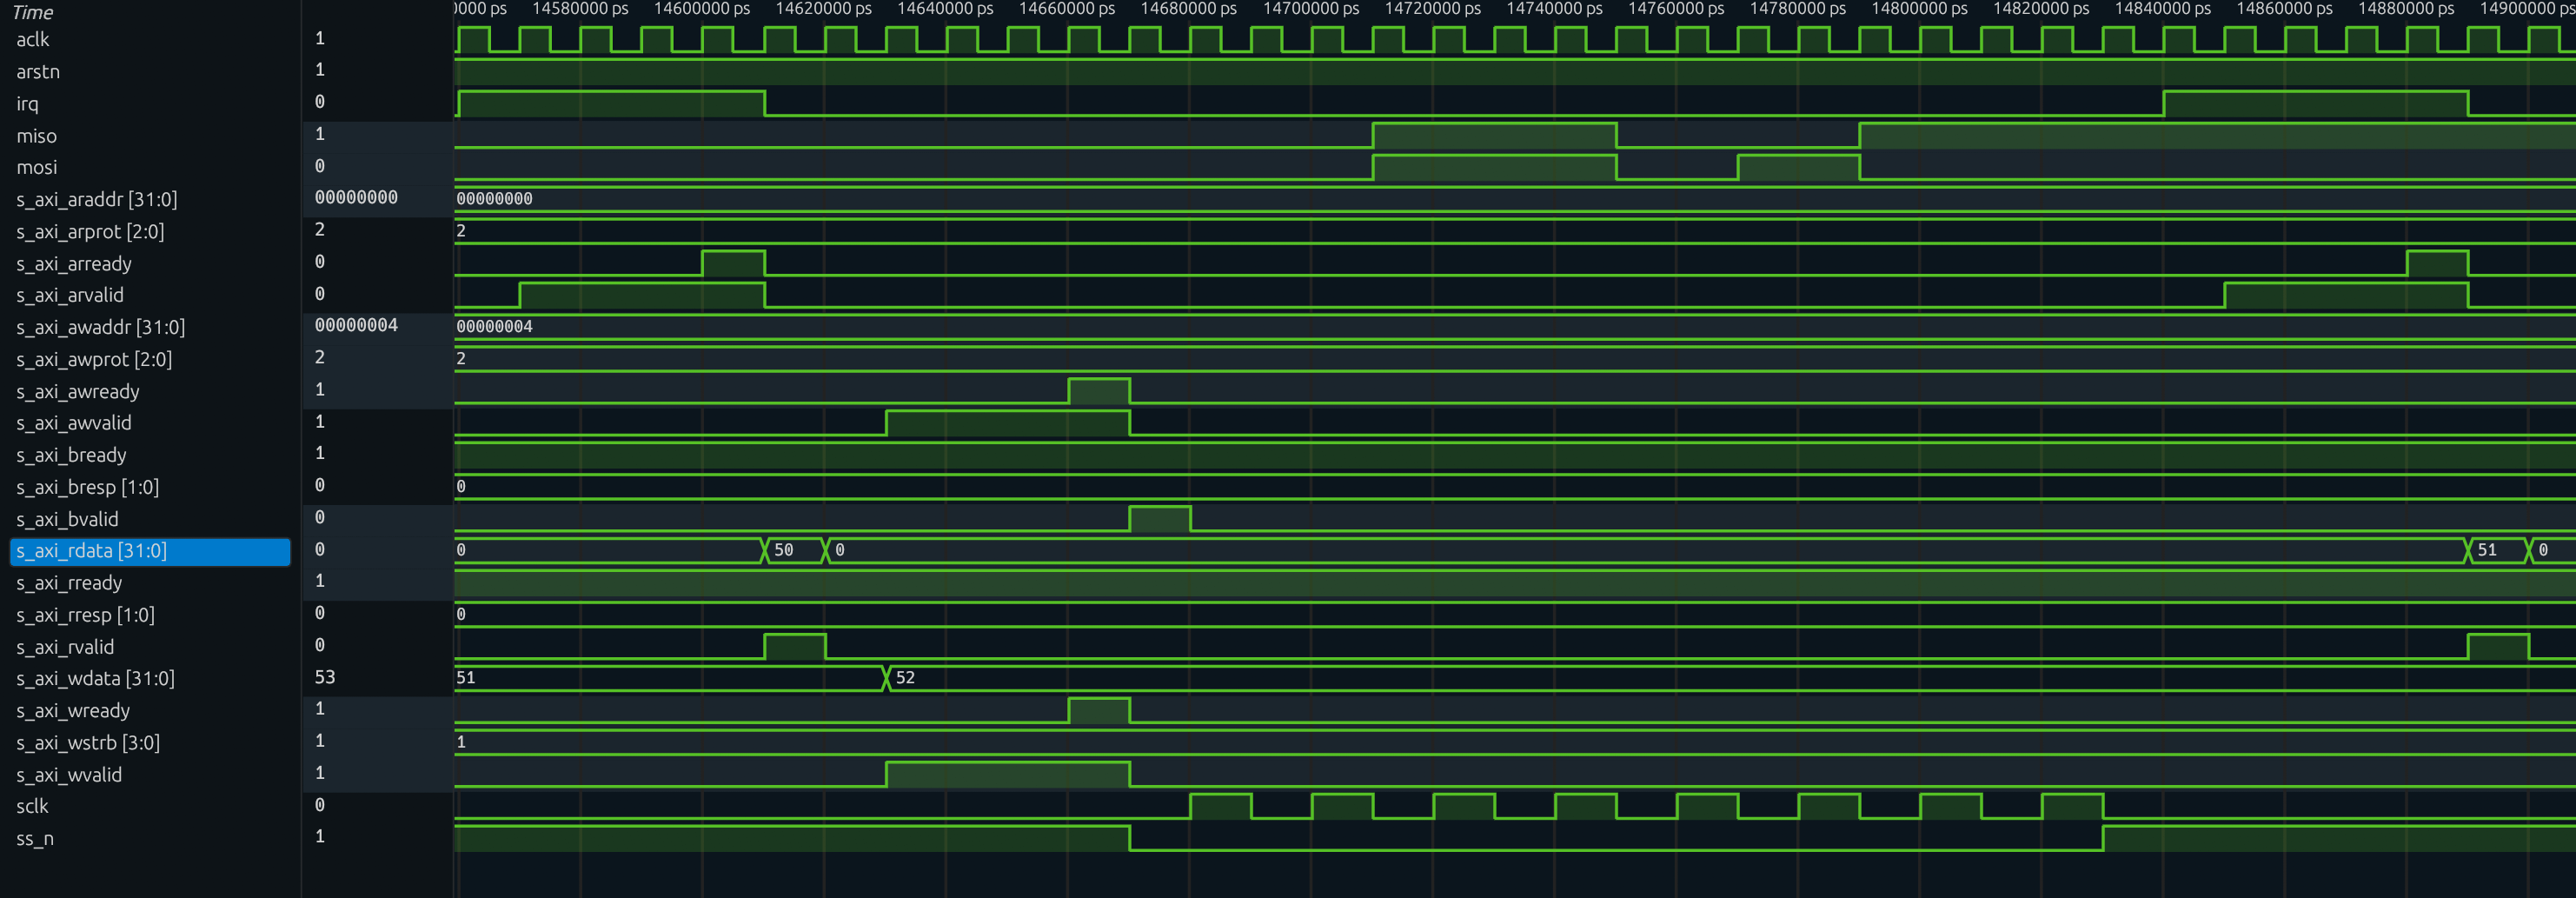
\includegraphics[width=\textwidth]{img/diagrams/waveform_loop_test_axil.png}
\end{figure}

\begin{figure}[H]
\caption{loop test wishbone standard}
\centering
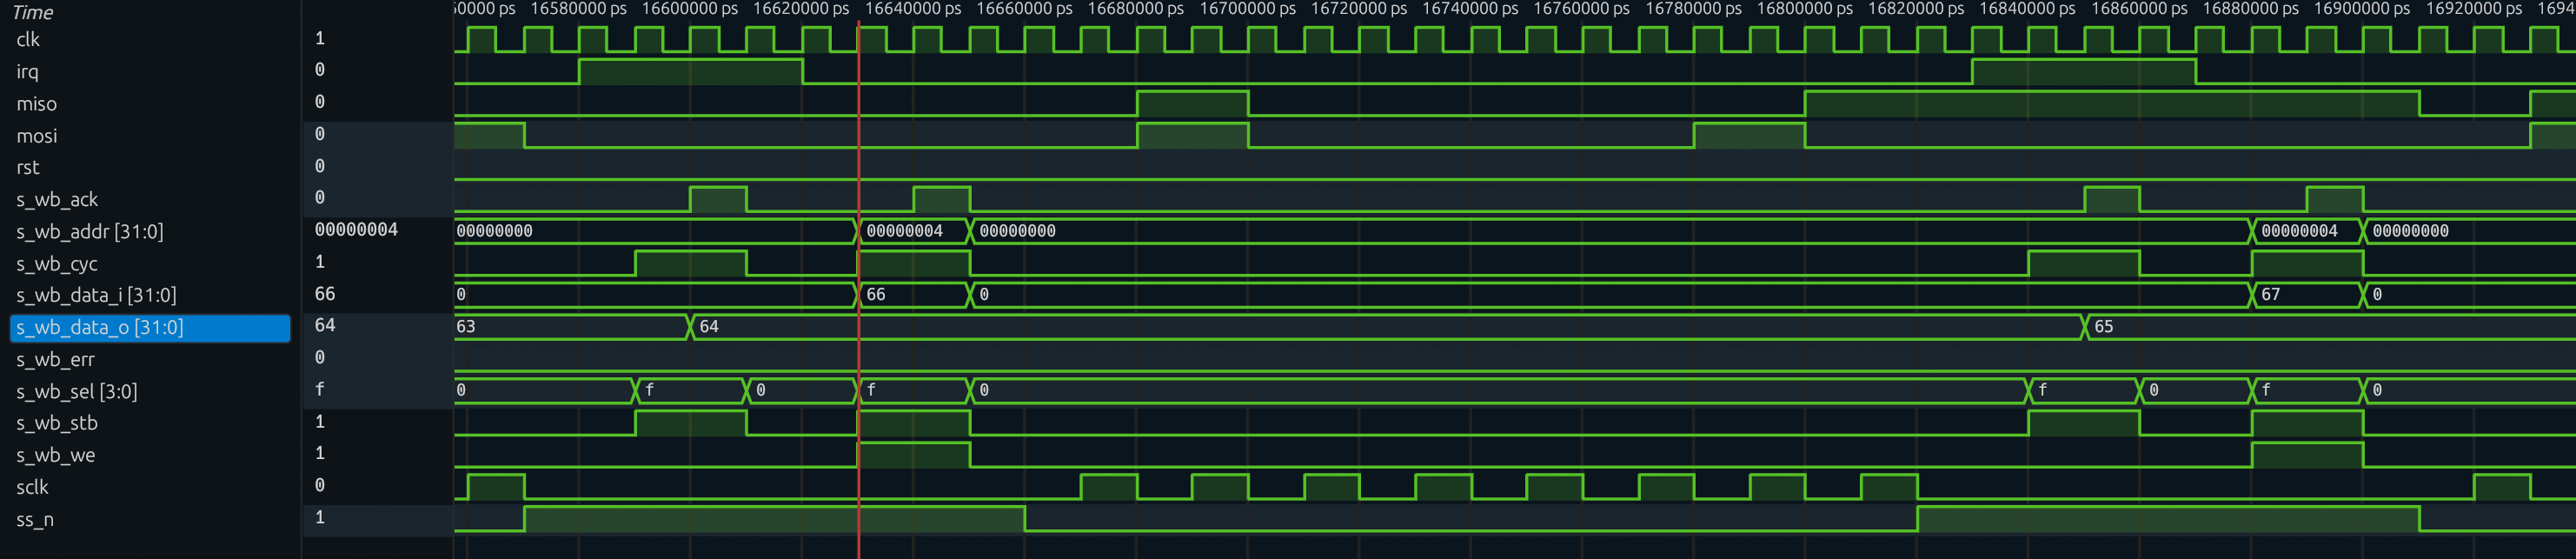
\includegraphics[width=\textwidth]{img/diagrams/waveform_loop_test_wishbone_standard.png}
\end{figure}

\section{Building}

\par
The BUS SPI MASTER is written in Verilog 2001. It should synthesize in any modern FPGA software. It comes as a fusesoc packaged core and can be included in any other core. Be sure to make sure you have meet the dependencies listed in the previous section. Linting is performed by verible using the lint target.

\subsection{fusesoc}
\par
Fusesoc is a system for building FPGA software without relying on the internal project management of the tool. Avoiding vendor lock in to Vivado or Quartus.
These cores, when included in a project, can be easily integrated and targets created based upon the end developer needs. The core by itself is not a part of
a system and should be integrated into a fusesoc based system. Simulations are setup to use fusesoc and are a part of its targets.

\subsection{Source Files}

\subsubsection{axi\_lite\_spi\_master File List}
\begin{itemize}
\item src
	\begin{itemize}
	\item src/axi\_lite\_spi\_master.v
	\end{itemize}
\item tb\_cocotb
	\begin{itemize}
	\item {'tb/tb\_cocotb\_axi\_lite.py': {'file\_type': 'user', 'copyto': '.'}}
	\item {'tb/tb\_cocotb\_axi\_lite.v': {'file\_type': 'verilogSource'}}
	\end{itemize}
\item tb
	\begin{itemize}
	\item tb/tb\_uart.v
	\end{itemize}
\end{itemize}


\subsubsection{wishbone\_standard\_spi\_master File List}
\begin{itemize}
\item src
	\begin{itemize}
	\item src/wishbone\_standard\_spi\_master.v
	\end{itemize}
\item tb\_cocotb
	\begin{itemize}
	\item {'tb/tb\_cocotb\_wishbone\_standard.py': {'file\_type': 'user', 'copyto': '.'}}
	\item {'tb/tb\_cocotb\_wishbone\_standard.v': {'file\_type': 'verilogSource'}}
	\end{itemize}
\end{itemize}


\subsubsection{up\_spi\_master File List}
\begin{itemize}
\item src
	\begin{itemize}
	\item src/up\_spi\_master.v
	\end{itemize}
\item tb\_cocotb
	\begin{itemize}
	\item {'tb/tb\_cocotb\_up.py': {'file\_type': 'user', 'copyto': '.'}}
	\item {'tb/tb\_cocotb\_up.v': {'file\_type': 'verilogSource'}}
	\end{itemize}
\end{itemize}


\subsection{Targets}

\subsubsection{axi\_lite\_spi\_master Targets}
\begin{itemize}
\item default
	\begin{itemize}
	\item[$\space$] Info: Default for IP intergration.
	\end{itemize}
\item sim\_cocotb
	\begin{itemize}
	\item[$\space$] Info: Cocotb unit tests
	\end{itemize}
\end{itemize}


\subsubsection{wishbone\_standard\_spi\_master Targets}
\begin{itemize}
\item default
	\begin{itemize}
	\item[$\space$] Info: Default for IP intergration.
	\end{itemize}
\item sim\_cocotb
	\begin{itemize}
	\item[$\space$] Info: Cocotb unit tests
	\end{itemize}
\end{itemize}


\subsubsection{up\_spi\_master Targets}
\begin{itemize}
\item default
	\begin{itemize}
	\item[$\space$] Info: Default for IP intergration.
	\end{itemize}
\item lint
	\begin{itemize}
	\item[$\space$] Info: Lint with Verible
	\end{itemize}
\item sim\_cocotb
	\begin{itemize}
	\item[$\space$] Info: Cocotb unit tests
	\end{itemize}
\end{itemize}


\subsection{Directory Guide}

\par
Below highlights important folders from the root of the directory.

\begin{enumerate}
  \item \textbf{docs} Contains all documentation related to this project.
    \begin{itemize}
      \item \textbf{manual} Contains user manual and github page that are generated from the latex sources.
    \end{itemize}
  \item \textbf{src} Contains source files for the core
  \item \textbf{tb} Contains test bench files for iverilog and cocotb
    \begin{itemize}
      \item \textbf{cocotb} testbench files
    \end{itemize}
\end{enumerate}

\newpage

\section{Simulation}
\par
There are a few different simulations that can be run for this core.

\subsection{cocotb}
\par
Cocotb is the only method for simulating the various interations of the bus\_spi\_master core. At the moment there is a
axi\_lite, wishbone\_standard, and uP based versions. This is currently set to use icarus as the sim tool for cocotb. The uP
testbench is the one that will test all the various register bits and interrupt options. Others will only do loop back tests.

\par
To run the wishbone sim use the command below.
\begin{lstlisting}[language=bash]
fusesoc run --target sim_cocotb AFRL:device:wishbone_standard_spi_master:1.0.0
\end{lstlisting}

\par
To run the axi\_lite sim use the command below.
\begin{lstlisting}[language=bash]
fusesoc run --target sim_cocotb AFRL:device:axi_lite_spi_master:1.0.0
\end{lstlisting}

\par
To run the uP sim use the command below.
\begin{lstlisting}[language=bash]
fusesoc run --target sim_cocotb AFRL:device:up_spi_master:1.0.0
\end{lstlisting}


\newpage

\section{Module Documentation} \label{Module Documentation}

\par
up\_spi\_master is the module that integrates the AXIS SPI MASTER core.
This uses inputs/outputs for data tied directly to registers mapped in the uP bus.
The uP bus is the microprocessor bus based on Analog Devices design. It resembles a APB bus in design,
and is the bridge to other buses BUS SPI MASTER can use. This makes changing for AXI Lite, to Wishbone to whatever
quick and painless.

\par
axi\_lite\_spi module adds a AXI Lite to uP (microprocessor) bus converter. The converter is
from Analog Devices.

\par
wishbone\_standard\_spi module adds a Wishbone Standard to uP (microprocessor) bus converter. This
converter was designed for Wishbone Standard only, NOT pipelined or Registered (cti).

\vspace{15mm}
\par
The next sections document these modules. up\_spi\_master contains the register map explained, and what the various bits do.

